\documentclass[12pt,a4paper]{article}
\usepackage{algorithm, algpseudocode, amsmath, amssymb, amsthm, bm, csquotes, emf, empheq, geometry, graphicx, hyperref, listings, mhchem, multirow, siunitx, slashbox, subcaption, upgreek}
\usepackage[italicdiff]{physics}
\usepackage[section]{placeins}
\usepackage[justification=centering]{caption}
\usepackage[column=O]{cellspace}
\usepackage[extrafootnotefeatures]{xepersian}
\hypersetup{colorlinks=true, urlcolor=cyan}

\title{تمرین سری دوازده دینامیک غیرخطی و آشوب}
\author{صالح شاملو احمدی}
\date{۷ خرداد ۱۴۰۲}

\settextfont{Yas}
\linespread{1.2}

\setlength\cellspacetoplimit{4pt}
\setlength\cellspacebottomlimit{3pt}
\newcommand{\multlinecell}[1]{\begin{tabular}[c]{@{}c@{}}#1\end{tabular}}

\newcommand{\qfrac}[2]{\left(\frac{#1}{#2}\right)}
\newcommand{\fsqrt}[2]{\sqrt{\frac{#1}{#2}}}
\newcommand{\ddfrac}[2]{{\displaystyle\frac{\displaystyle #1}{\displaystyle #2}}}
\newcommand{\pdvc}[3]{\qfrac{\partial #1}{\partial #2}_{#3}}
\newcommand{\dbar}{{d\mkern-7mu\mathchar'26\mkern-2mu}}
\newcommand*{\defeq}{\mathrel{\vcenter{\baselineskip0.5ex \lineskiplimit0pt
			\hbox{\scriptsize.}\hbox{\scriptsize.}}}
	=}

\newtheorem{theorem}{قضیه}
\newtheorem{lemma}{لم}
\renewcommand\qedsymbol{$\blacksquare$}

\begin{document}
	\maketitle
	\section{مسئله \lr{9.2.1}}
	\subsection{\lr{a}}
	برای پیدا کردن $C^{\pm}$ باید سیستم معادلات
	$(\dot{x}, \dot{y}, \dot{z}) = (0, 0, 0)$
	را حل کنیم. یعنی
	\begin{subequations}
		\begin{empheq}[left=\empheqlbrace]{align}
			\sigma(y-x) &= 0, \\
			rx - xz - y &= 0, \\
			xy - bz &= 0,
		\end{empheq}
	\end{subequations}
	پس، به ترتیب از معادله اول تا سوم نتیجه می‌گیریم
	\begin{align}
		x &= y, \\
		z &= r - 1, \\
		x &= y = \pm\sqrt{b(r - 1)}.
	\end{align}
	پس در کل
	\begin{equation}
		C^{\pm} = \qty(\pm\sqrt{b(r-1)}, \pm\sqrt{b(r-1)}, r - 1).
	\end{equation}
	حال ماتریس ژاکوبی را محاسبه می‌کنیم.
	\begin{equation}
		J = \mqty(-\sigma & \sigma & 0 \\ r - z & -1 & -x \\ y & x & -b) \implies
		J_{C^{\pm}} = \mqty(-\sigma & \sigma & 0 \\ 1 & -1 & \mp\sqrt{b(r-1)} \\ \pm\sqrt{b(r-1)} & \pm\sqrt{b(r-1)} & -b)
	\end{equation}
	معادله مشخصه ویژه مقادیر این ماتریس از $\det(J_{C^{\pm}} - \lambda \mathbb{I}) = 0 $ بدست می‌آید.
	\begin{gather}
		\det\mqty(-\sigma-\lambda & \sigma & 0 \\ 1 & -1-\lambda & \mp\sqrt{b(r-1)} \\ \pm\sqrt{b(r-1)} & \pm\sqrt{b(r-1)} & -b-\lambda) = 0 \\
		(-\sigma-\lambda)\qty[(-1 - \lambda)(-b - \lambda) + b(r-1)] - \sigma\qty[(-b-\lambda) + b(r-1)] = 0 \\
		\lambda^3 + (\sigma + b + 1)\lambda^2 + b(\sigma + r)\lambda + 2\sigma b(r-1) = 0
	\end{gather}

	\subsection{\lr{b}}
	\begin{equation}
		-i\omega^3 - (\sigma + b + 1)\omega^2 + ib(\sigma + r)\omega + 2\sigma b(r-1) = 0
	\end{equation}
	با جداسازی بخش حقیقی و موهومی،
	\begin{empheq}[left=\empheqlbrace]{gather}
		-\omega^3 + b(\sigma + r)\omega = 0 \\
		-(\sigma + b + 1)\omega^2 + 2\sigma b(r-1) = 0
	\end{empheq}
	تنها راهی که هر دو معادله همزمان برقرار باشند، باید $\omega^2 $ی که از دو معادله بدست می‌آید را برابر قرار دهیم. پس
	\begin{equation}
		b(\sigma + r) = \frac{2\sigma b(r-1)}{\sigma + b + 1}.
	\end{equation}
	حال این معادله را برای $r$ حل می‌کنیم.
	\begin{gather}
		b(\sigma + r_H)(\sigma + b + 1) = 2\sigma b(r_H - 1) \\
		r_H = \frac{\sigma + b + 3}{\sigma - b - 1}
	\end{gather}
	چون $r>0 $، برای پیدا شدن $r = r_H$ باید $\sigma > b + 1 $.
	\subsection{\lr{c}}
	\begin{align}
		\omega = \pm\omega_0 = \pm\sqrt{b(\sigma + r)}
		&\implies (\lambda - i\omega_0)(\lambda + i\omega_0)(\lambda - \lambda_3) = 0 \\
		\qty(\lambda^2 - \omega_0^2)(\lambda - \lambda_3) = 0
		&\implies \qty[\lambda^2 - b(\sigma + r)](\lambda - \lambda_3) = 0 \\
		\lambda^3 - \lambda_3\lambda^2 &- b(\sigma + r)\lambda + b\lambda_3(\sigma + r) = 0
	\end{align}
	با مقایسه این رابطه با معادله مشخصه،
	\begin{empheq}[box=\fbox]{equation}
		\lambda_3 = -(\sigma + b + 1).
	\end{empheq}

	\section{مسئله \lr{10.3.6}}
	\begin{equation}
		x_{n+1} = f(x_n) = rx_n - x_n^3
	\end{equation}

	\subsection{\lr{a}}
	\begin{empheq}[left={x^* = rx^* - x^{*3}\implies\empheqlbrace}]{align}
		x^* &= 0;\quad\text{همه $r$های ممکن} \\
		x^* &= \pm\sqrt{r-1};\quad r>1
	\end{empheq}
	\begin{empheq}[left={f'(x) = r - 3x^2 \implies\empheqlbrace}]{align}
		f'(0) &= r \\
		f'\qty(\pm\sqrt{r-1}) &= 3 - 2r
	\end{empheq}
	اگر $\abs{f'(x)}>1 $، نقطه ثابت ناپایدار و اگر $\abs{f'(x)}<1 $، نقطه ثابت پایدار است.
	\begin{empheq}[left={x^* = 0 \empheqlbrace}]{align}
		\abs{r} &< 1:\quad\text{پایدار} \\
		\abs{r} &> 1:\quad\text{ناپایدار}
	\end{empheq}
	\begin{empheq}[left={x^* = \pm\sqrt{r-1} \empheqlbrace}]{align}
		1 < r < 2 &:\quad\text{پایدار} \\
		r > 2,\ r<1 &:\quad\text{ناپایدار}
	\end{empheq}

	\subsection{\lr{b}}
	$p$ و $q$ جواب‌های معادله $x = f(f(x))$ هستند که معادل است با
	\begin{gather}
		x = r\qty(rx - x^3) - \qty(rx - x^3)^3, \\
		x\qty[\qty(r - x^2)\qty(r - x^2\qty(r-x^2)^2) - 1] = 0.
	\end{gather}
	برای فاکتورگیری و ساده‌سازی، تعریف می‌کنیم $u \defeq r - x^2 $. در این صورت
	\begin{equation}
		x\qty[u\qty(r - x^2u^2) - 1] = 0.
	\end{equation}
	با حذف $r$ از معادله،
	\begin{align}
		x\qty[u\qty(u + x^2 - x^2u^2) - 1] &= 0, \\
		x\qty[u^2 - 1 + ux^2(1 - u^2)] &= 0, \\
		x\qty(u^2 - 1)\qty(1 - ux^2) &= 0, \\
		x\qty(u - 1)(u + 1)\qty(1 - ux^2) &= 0
	\end{align}
	با ضرب دو منفی در عبارات مزدوج و باز کردن $u$ برحسب $x$ و $r$،
	\begin{equation}
		x\qty(x^2 - r + 1)\qty(x^2 - r - 1)\qty(x^4 - rx^2 + 1) = 0.
	\end{equation}
	سه جمله اول این عبارت نقاط ثابت را می‌دهند، جز حالتی که
	$(p, q) = \qty(-\sqrt{1+r}, \sqrt{1+r})$.
	پس بقیه $p$ و $q$ جواب‌های جمله آخر هستند. آن‌ها عبارتند از
	\begin{align}
		(p, q) = \pm\qty(\fsqrt{r+\sqrt{r^2-4}}{2}, \fsqrt{r-\sqrt{r^2-4}}{2})
	\end{align}
	
	\subsection{\lr{c}}
	\begin{align}
		\dv{x}f(f(x)) &= f'(x)f'(f(x)) = f'(p)f'(q) \\
		&= \qty(r - 3p^2)\qty(r - 3q^2) \\
		&= r^2 -3r(p^2 + q^2) + 9p^2q^2
	\end{align}
	\begin{equation}
		(p, q) = \qty(-\sqrt{1+r}, \sqrt{1+r}):\ \dv{x}f(f(x)) = (2r + 3)^2 \ge 0
	\end{equation}
	چون در $r<-1 $ مقدار ریشه‌های موهومی می‌شود و برای اینکه قدر مطلق $\displaystyle\dv{x}f(f(x))$ از یک کوچک‌تر باشد،
	باید حتماً $r$ از $-1$ کوچک‌تر باشد، در تمام حالات این چرخه ناپایدار است.
	\begin{subequations}
		\begin{empheq}[left={(p, q) = \pm\qty(\sqrt{\ddfrac{r+\sqrt{r^2-4}}{2}}, \sqrt{\ddfrac{r-\sqrt{r^2-4}}{2}}) \empheqlbrace}]{align}
			p^2 + q^2 &= r \\
			p^2q^2 &= 1
		\end{empheq}
	\end{subequations}
	\begin{equation}
		\implies \dv{x}f(f(x)) = -2r^2 + 9
	\end{equation}
	شرط پایدار بودن این است که قدر مطلق این تابع از یک کوچک‌تر باشد، یا به عبارتی دیگر
	بین منفی یک و یک باشد. بنابراین در این $p$ و $q$
	\begin{subequations}
		\begin{empheq}[left=\empheqlbrace]{align}
			2 < \abs{r} < 5 &\implies \text{پایدار} \\
			\abs{r} < 2,\quad \abs{r} > 5 &\implies \text{ناپایدار}
		\end{empheq}
	\end{subequations}
	\subsection{\lr{d}}
	\begin{figure}[h!]
		\centering
		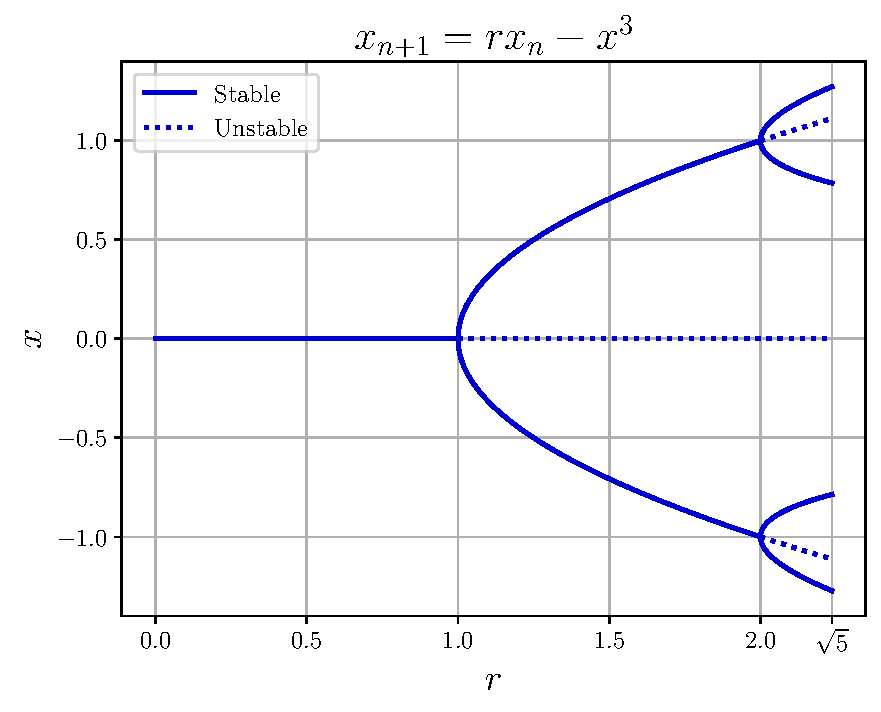
\includegraphics{fig/10.3.6.d}
		\caption{نمودار دوشاخگی تا $r$ بررسی‌شده}
	\end{figure}
	\section{نگاشت لورنتس}
	\subsection{آ و ب}
	مقادیر $\sigma = 8 $ و $b = 2 $ را انتخاب می‌کنیم. در این حالت $r_H = 20.8 $. در $r > r_H$ هنگامی که بیرون چرخه
	حدی قرار بگیریم، رباینده عجیب داریم که در $r > r_H$ در حالی که $r$ زیاد هم بزرگ نباشد، همواره این شرط برقرار است.
	\begin{figure}[h!]
		\centering
		\begin{LTR}
			\begin{subfigure}{0.49\linewidth}
				\centering
				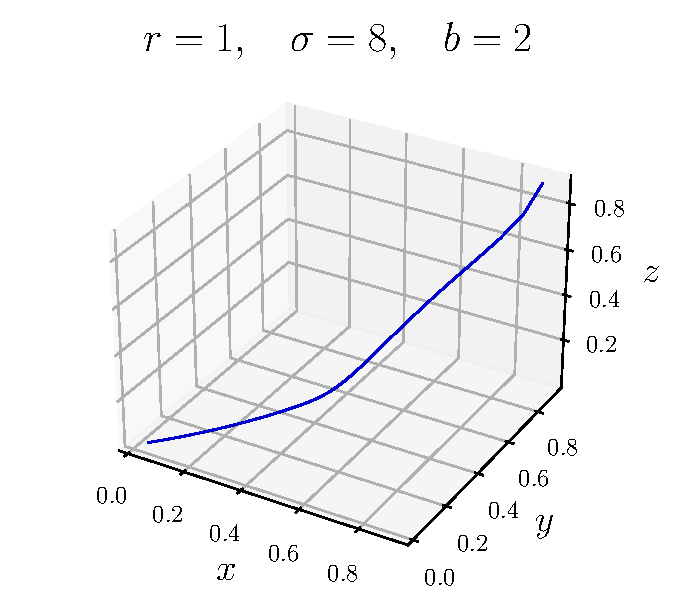
\includegraphics[width=\linewidth]{fig/lorenz1-3d}
			\end{subfigure}
			\begin{subfigure}{0.49\linewidth}
				\centering
				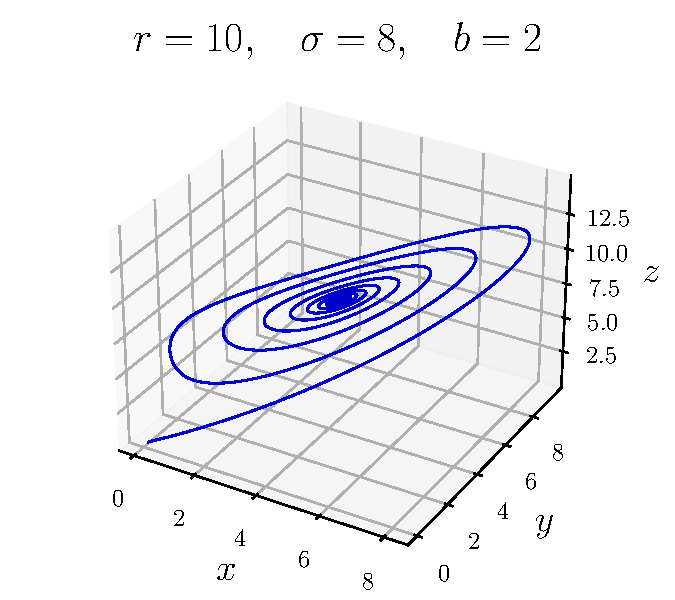
\includegraphics[width=\linewidth]{fig/lorenz2-3d}
			\end{subfigure}
			\begin{subfigure}{0.49\linewidth}
				\centering
				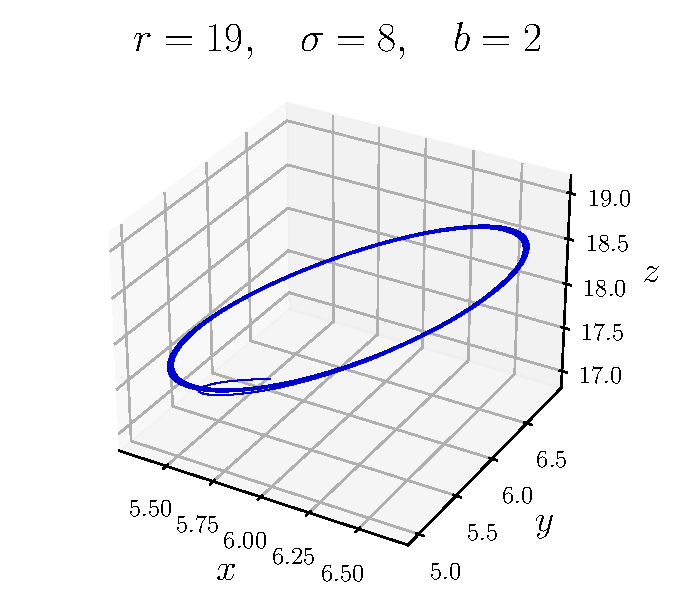
\includegraphics[width=\linewidth]{fig/lorenz3-3d}
			\end{subfigure}
			\begin{subfigure}{0.49\linewidth}
				\centering
				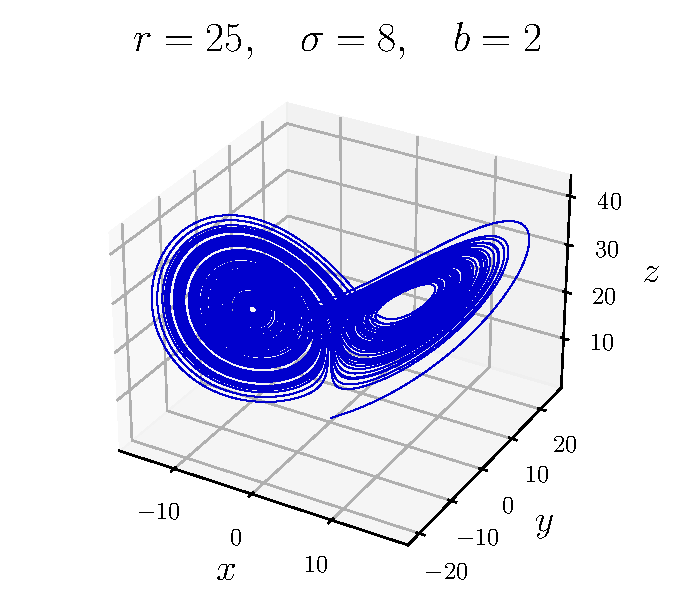
\includegraphics[width=\linewidth]{fig/lorenz4-3d}
			\end{subfigure}
		\end{LTR}
		\caption{نمودار سه‌بُعدی نگاشت لورنتس به ازای $r$های مختلف.}
	\end{figure}
	\newgeometry{left=0.1in, right=0.1in, top=0.3in, bottom=0.3in}
	\begin{figure}
		\centering
		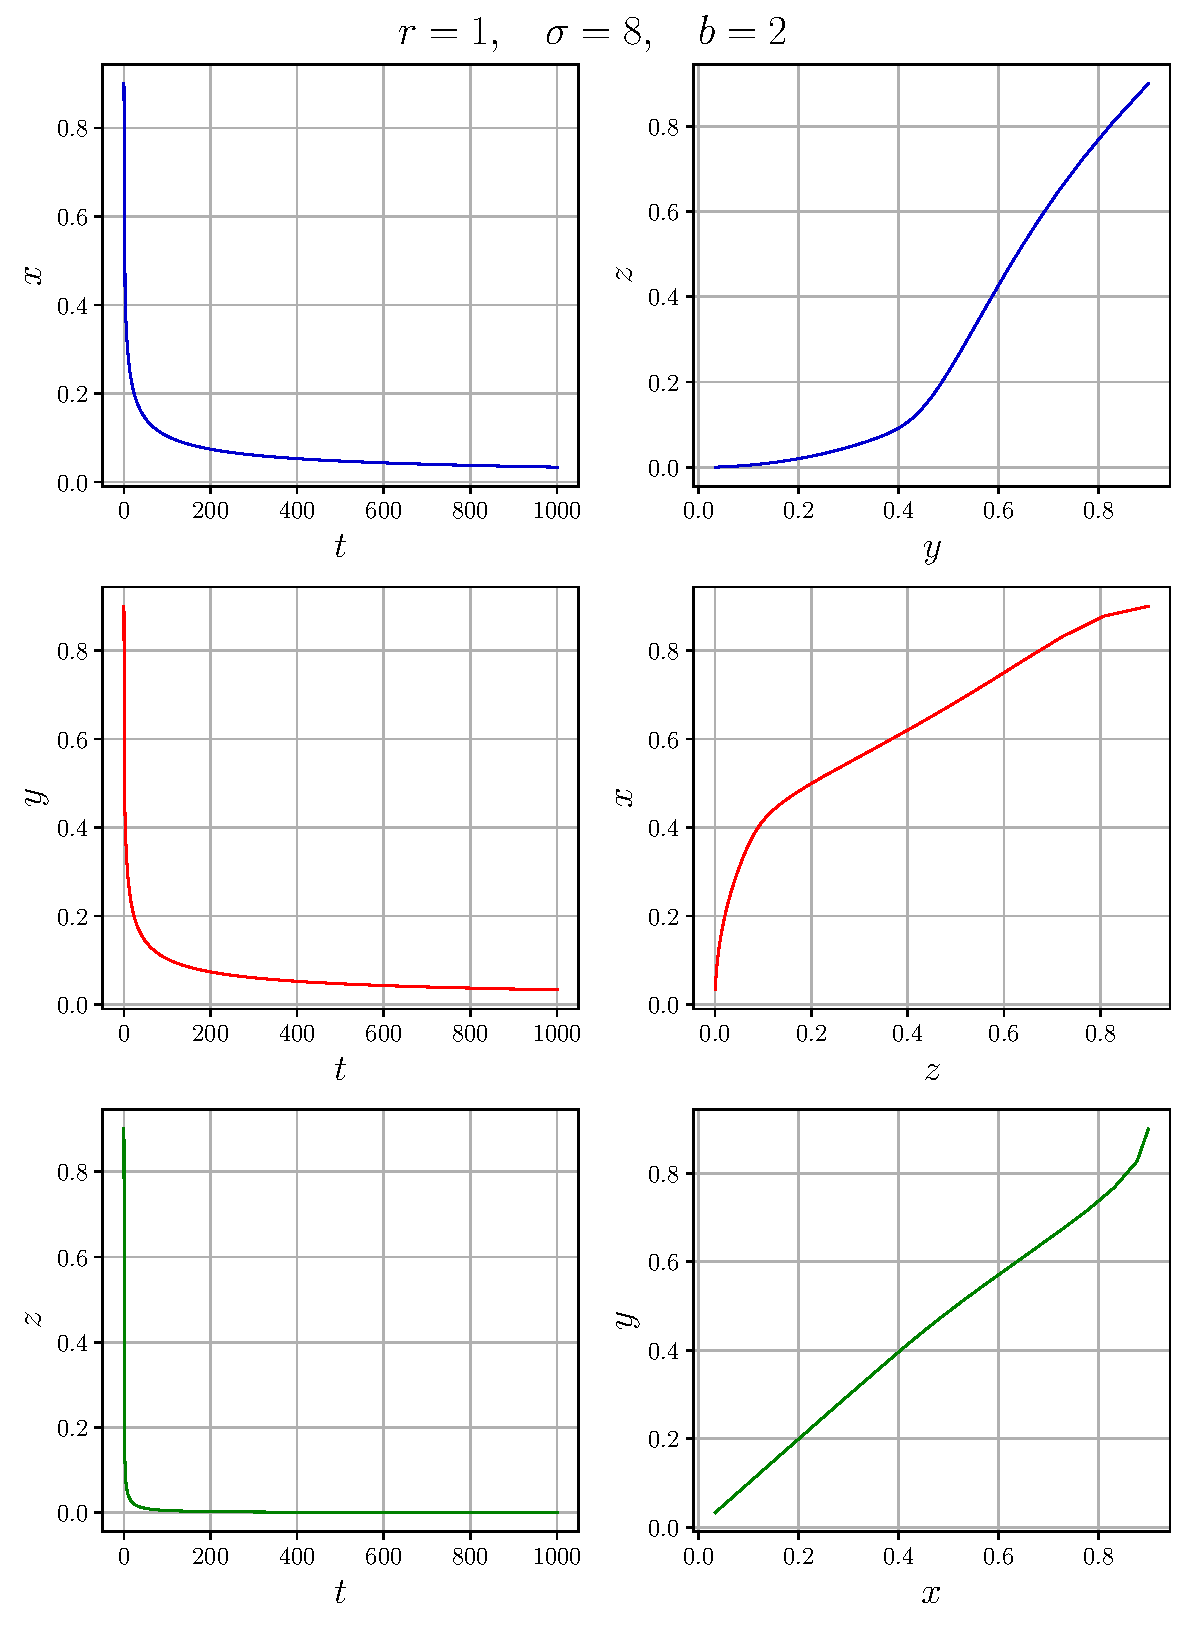
\includegraphics{fig/lorenz1}
	\end{figure}
	\begin{figure}
		\centering
		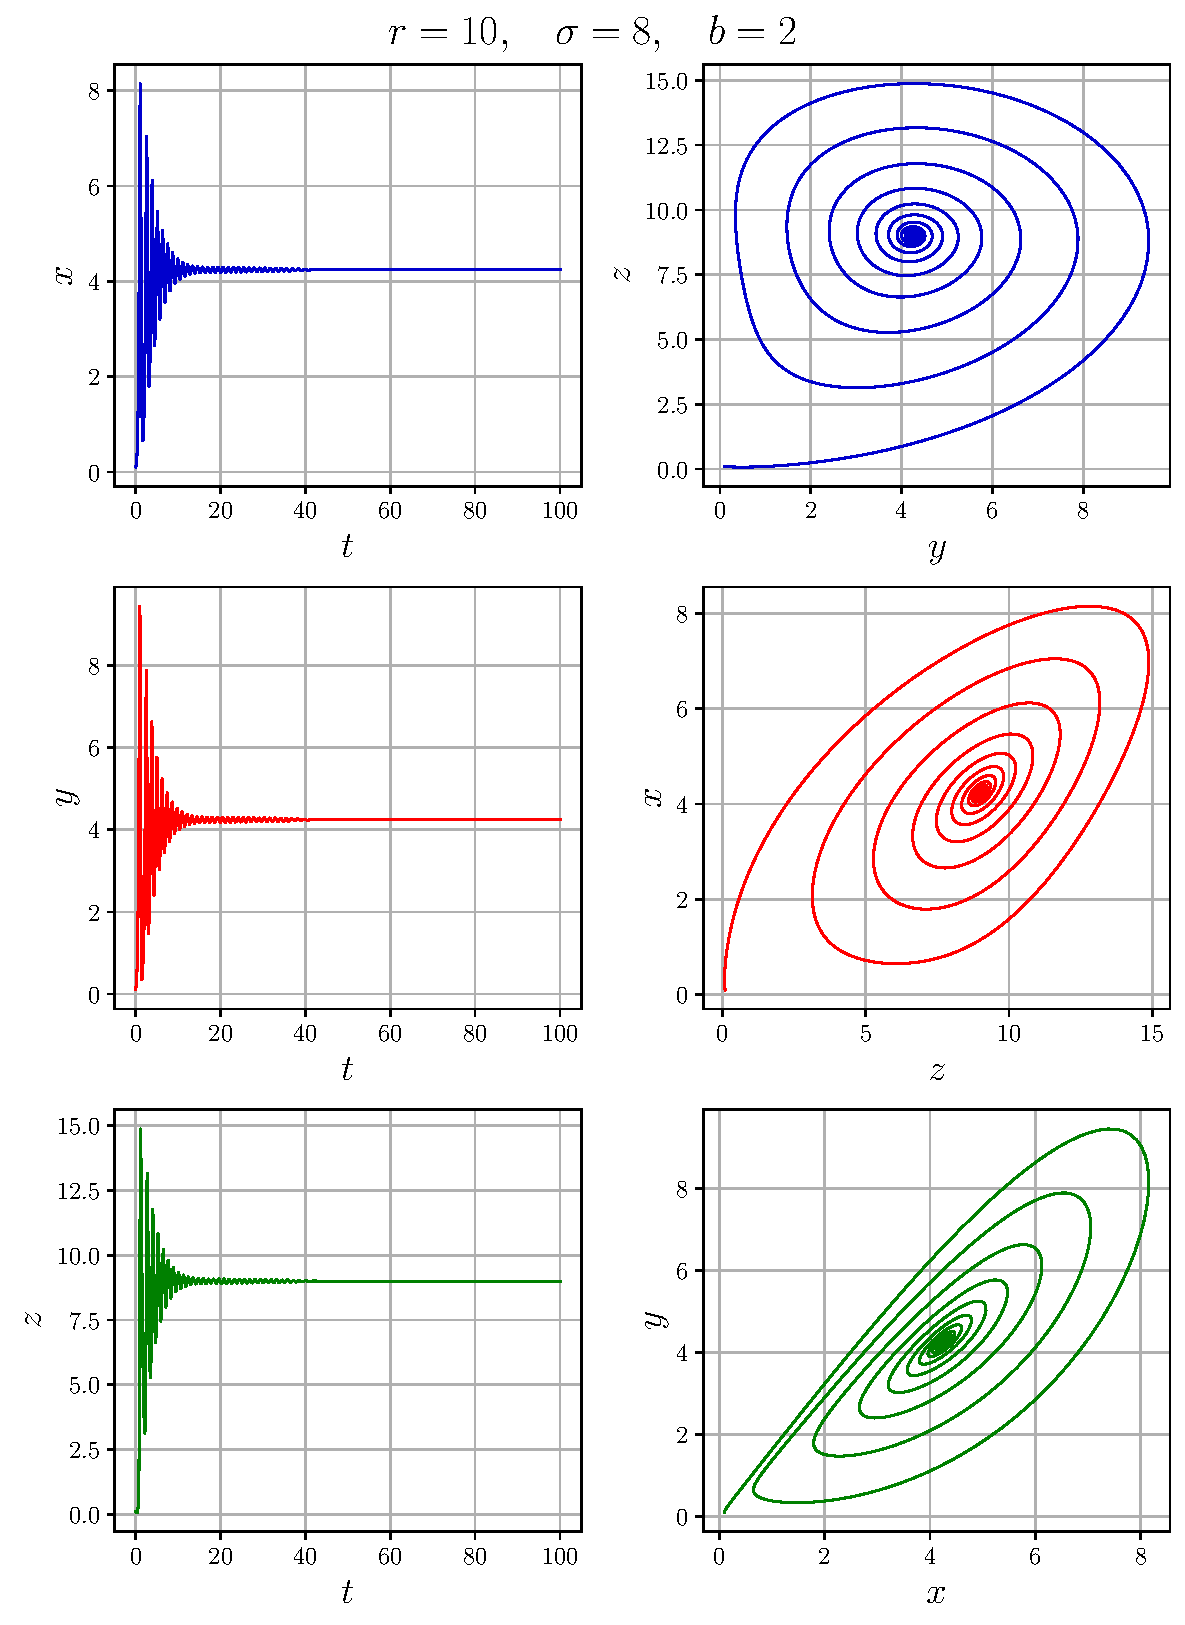
\includegraphics{fig/lorenz2}
	\end{figure}
	\begin{figure}
		\centering
		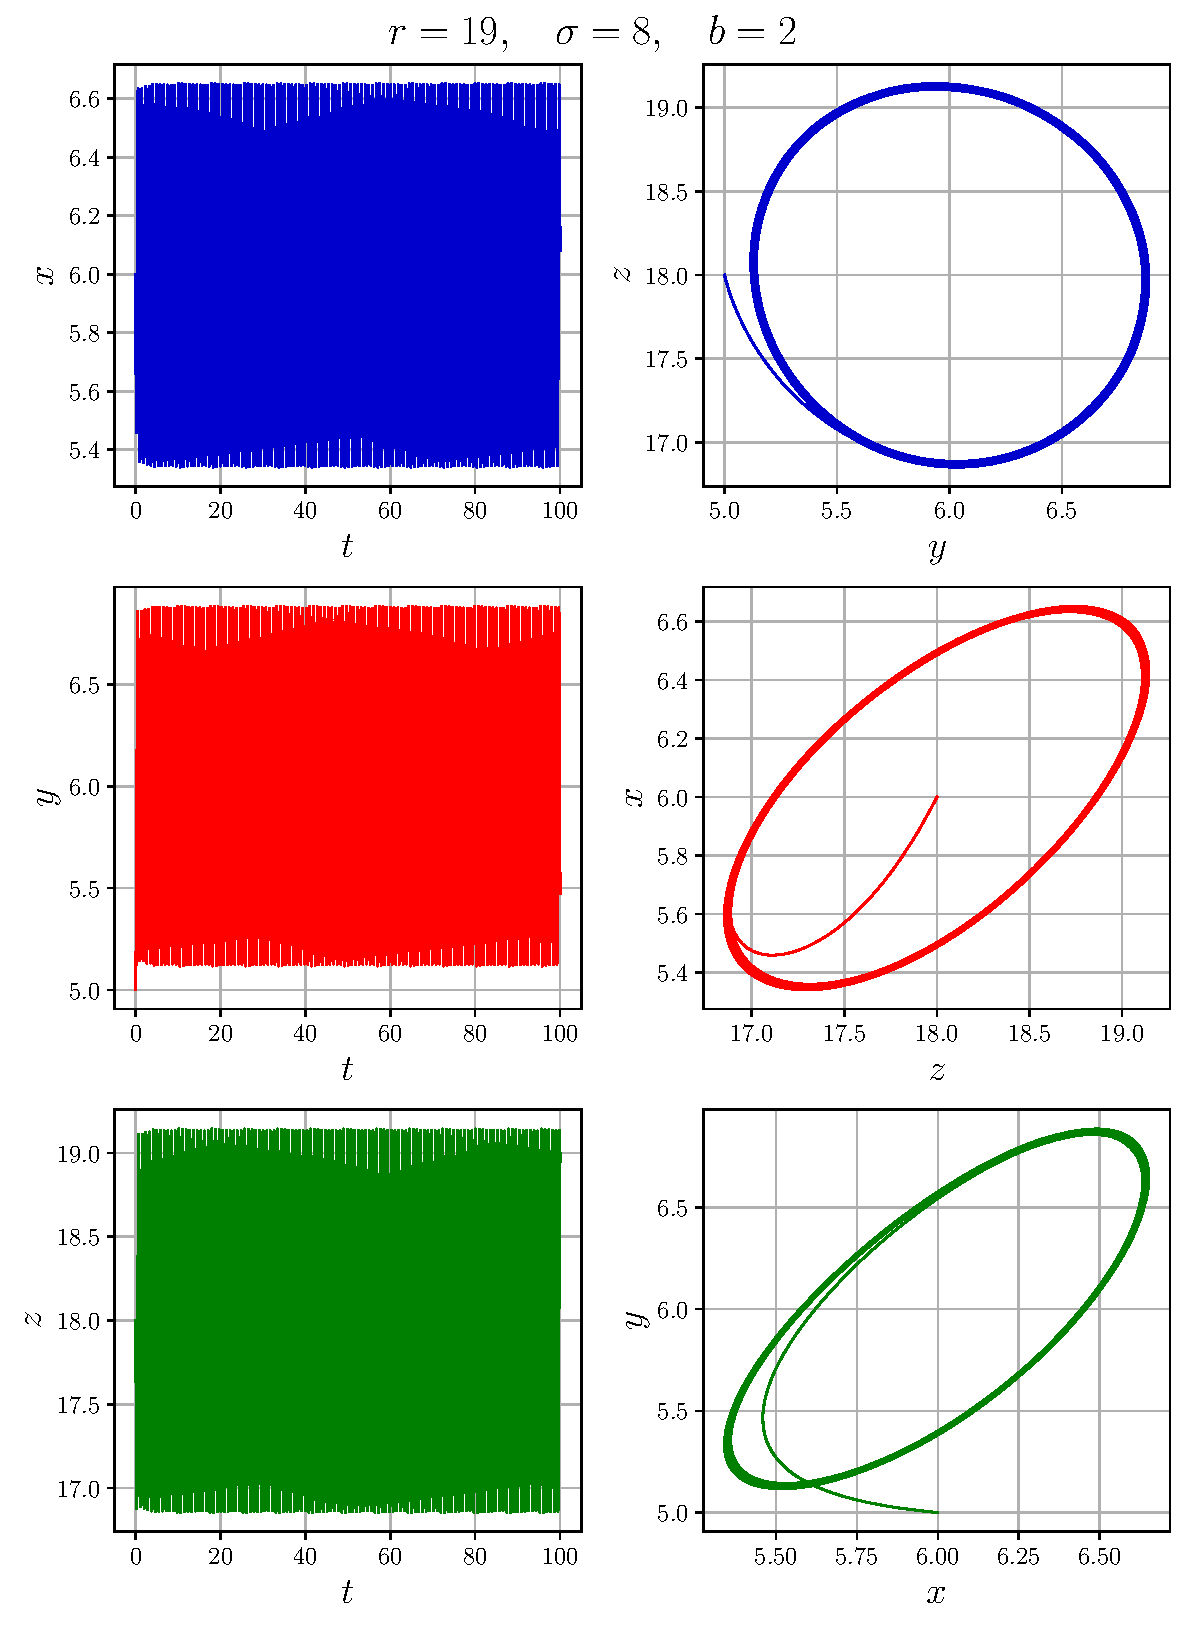
\includegraphics{fig/lorenz3}
	\end{figure}
	\begin{figure}
		\centering
		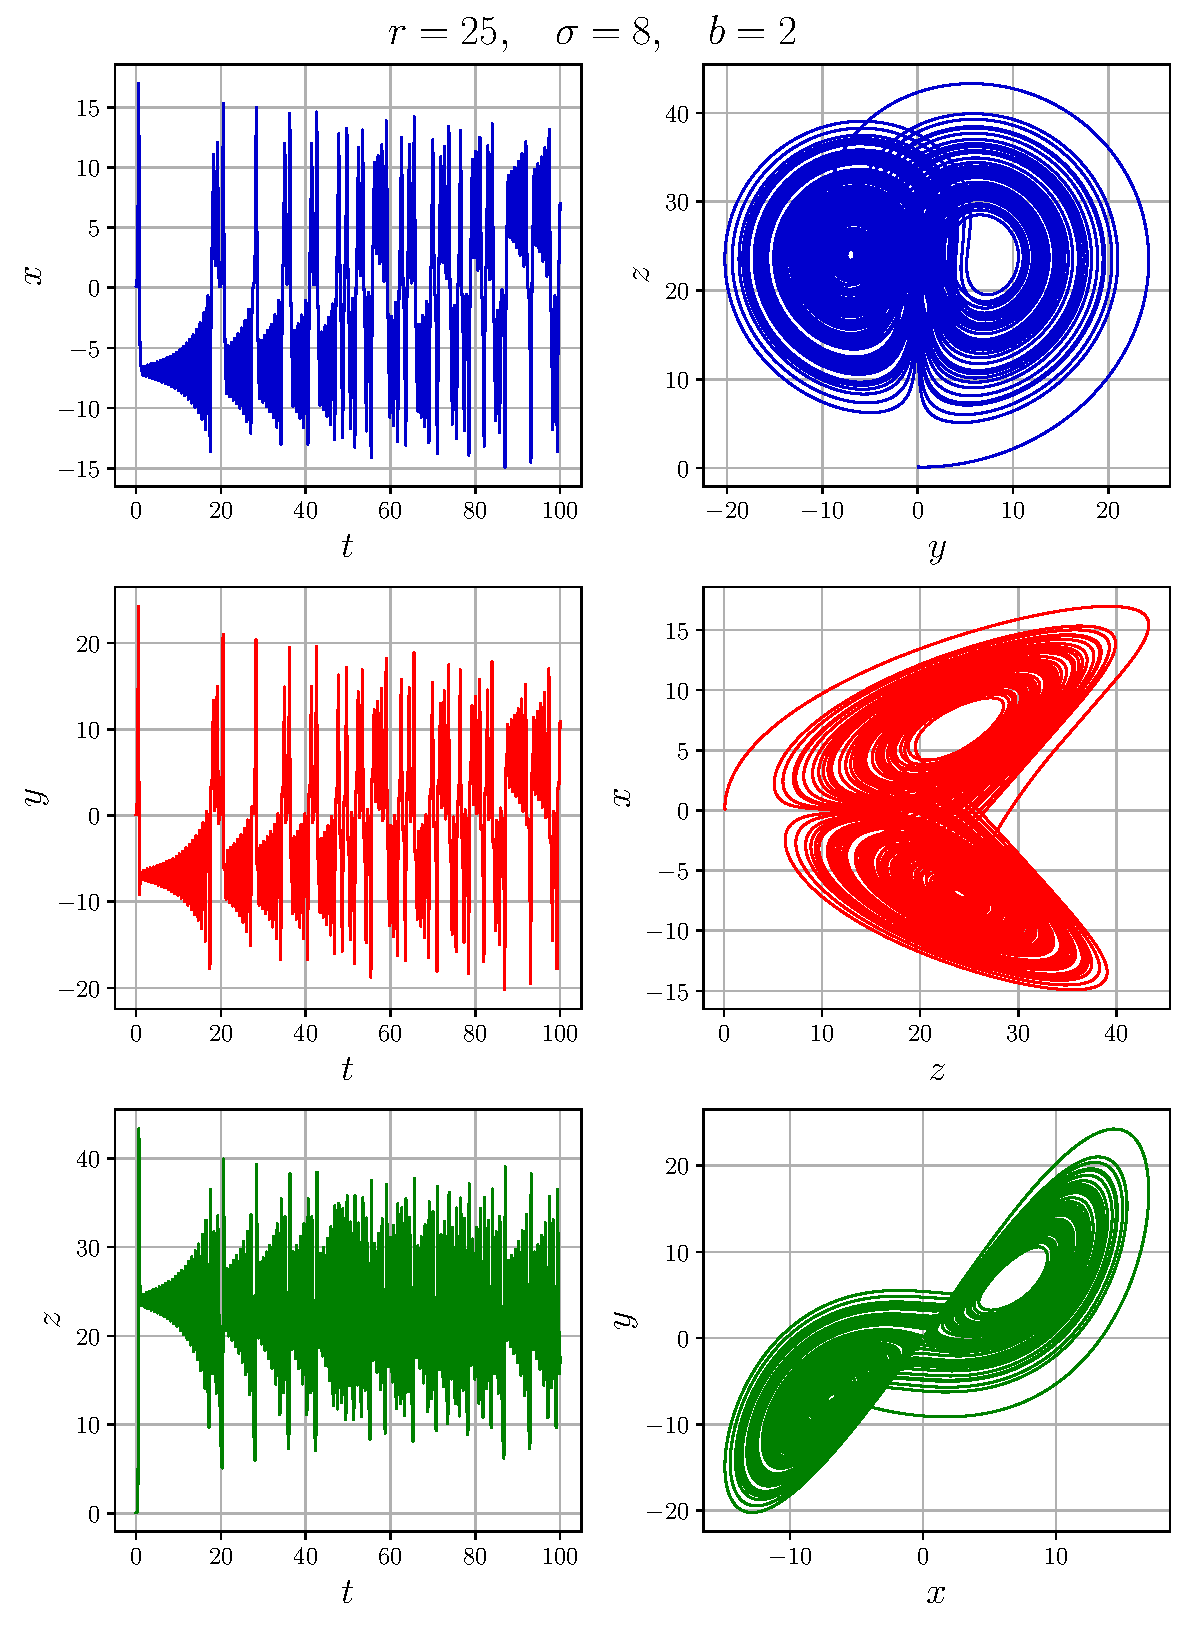
\includegraphics{fig/lorenz4}
	\end{figure}
	\restoregeometry
	\subsection{پ}
	از کُد استفاده‌شده در سری تمرین قبلی دوباره استفاده کردم. بدست می‌آید که $\lambda\approx1.06 $.
	\subsection{ت}
	\begin{figure}[h!]
		\centering
		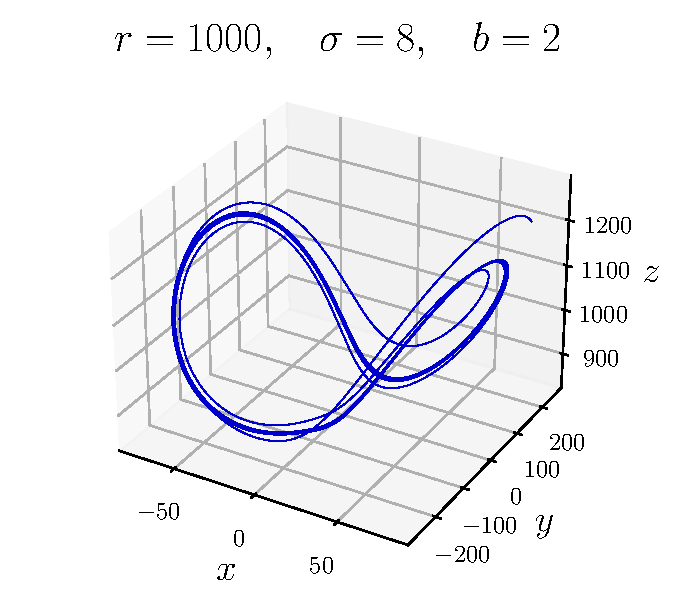
\includegraphics[width=\linewidth]{fig/lorenz5-3d}
	\end{figure}
	\newgeometry{left=0.1in, right=0.1in, top=0.3in, bottom=0.3in}
	\begin{figure}
		\centering
		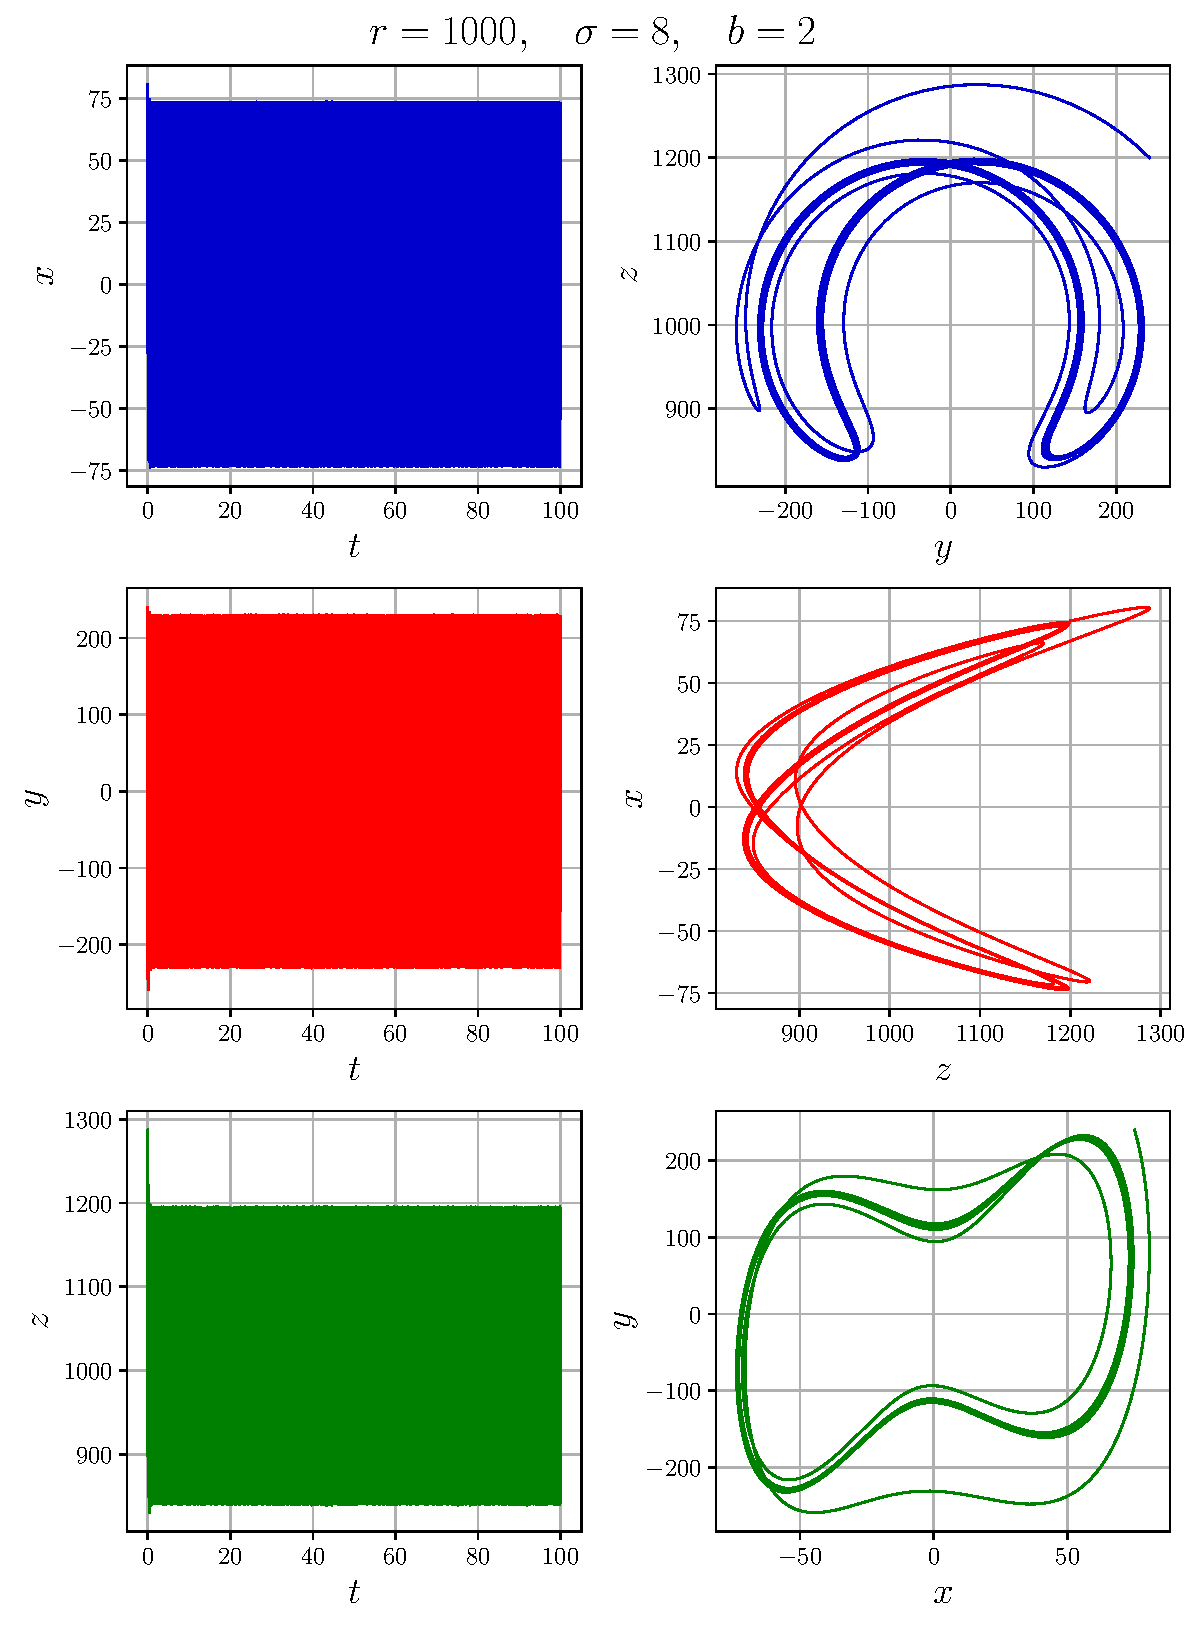
\includegraphics{fig/lorenz5}
	\end{figure}
	\restoregeometry
\end{document}